The dictator and proposer distributions show the answers under each card, separately by model. The saved heading also reports pooled P1.

\begin{figure*}[t]
\centering
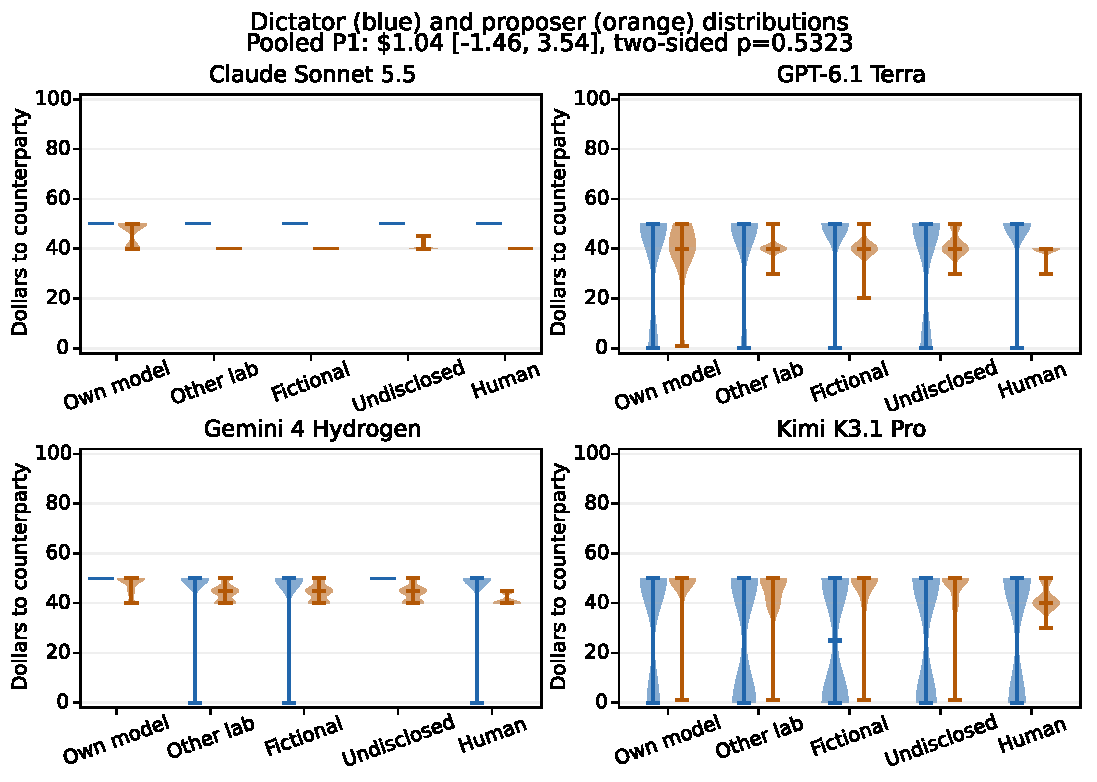
\includegraphics[width=\textwidth]{appendix/figures/study1-main_distributions.pdf}
\caption{Study 1 dictator (blue) and proposer (orange) distributions.}
\label{fig:appendix-study1-main_distributions}
\end{figure*}

The responder plot shows the minimum amounts required under each card. Each panel concerns a different model.

\begin{figure*}[t]
\centering
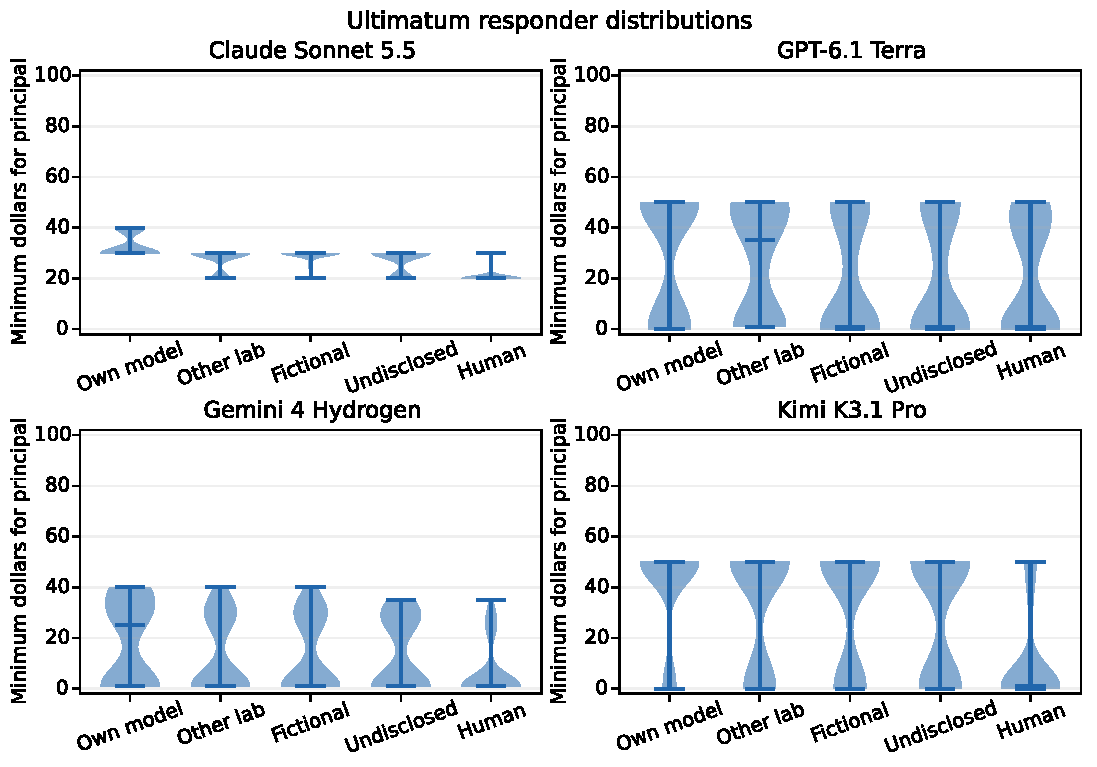
\includegraphics[width=\textwidth]{appendix/figures/study1-responder_distributions.pdf}
\caption{Study 1 ultimatum responder distributions.}
\label{fig:appendix-study1-responder_distributions}
\end{figure*}

This plot places the unadjusted offer, belief-adjusted offer and stated-belief contrasts side by side. Their comparison is descriptive rather than causal.

\begin{figure*}[t]
\centering
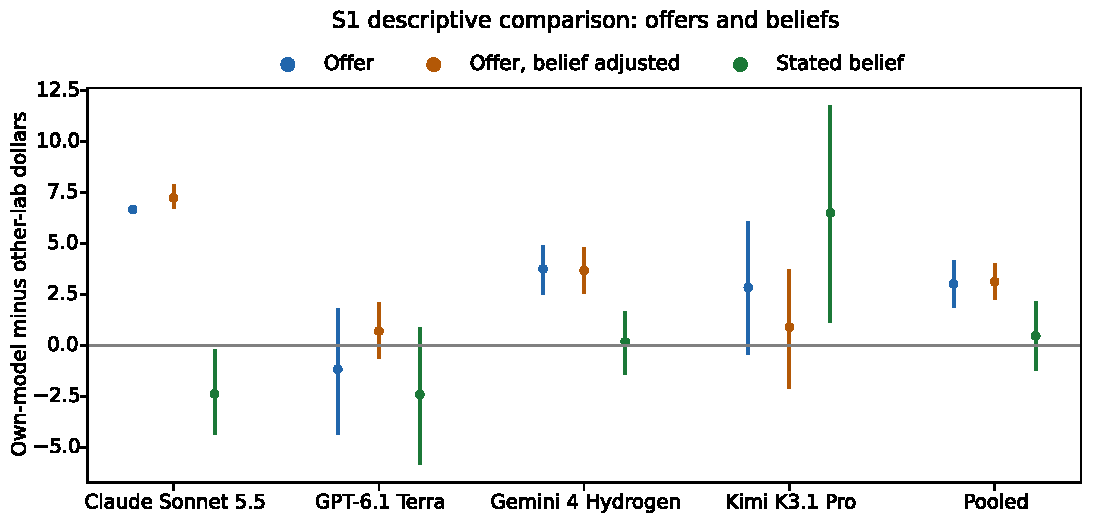
\includegraphics[width=\textwidth]{appendix/figures/study1-s1_coefficients.pdf}
\caption{Study 1 S1 contrasts: own model minus other lab, in dollars. Blue denotes the offer, orange the belief-adjusted offer, and green the stated belief.}
\label{fig:appendix-study1-s1_coefficients}
\end{figure*}

The registered check figure retains the yes, no and unsure counts and identifies which cards are scored. It describes a separate task, not decisions about money.

\begin{figure*}[t]
\centering
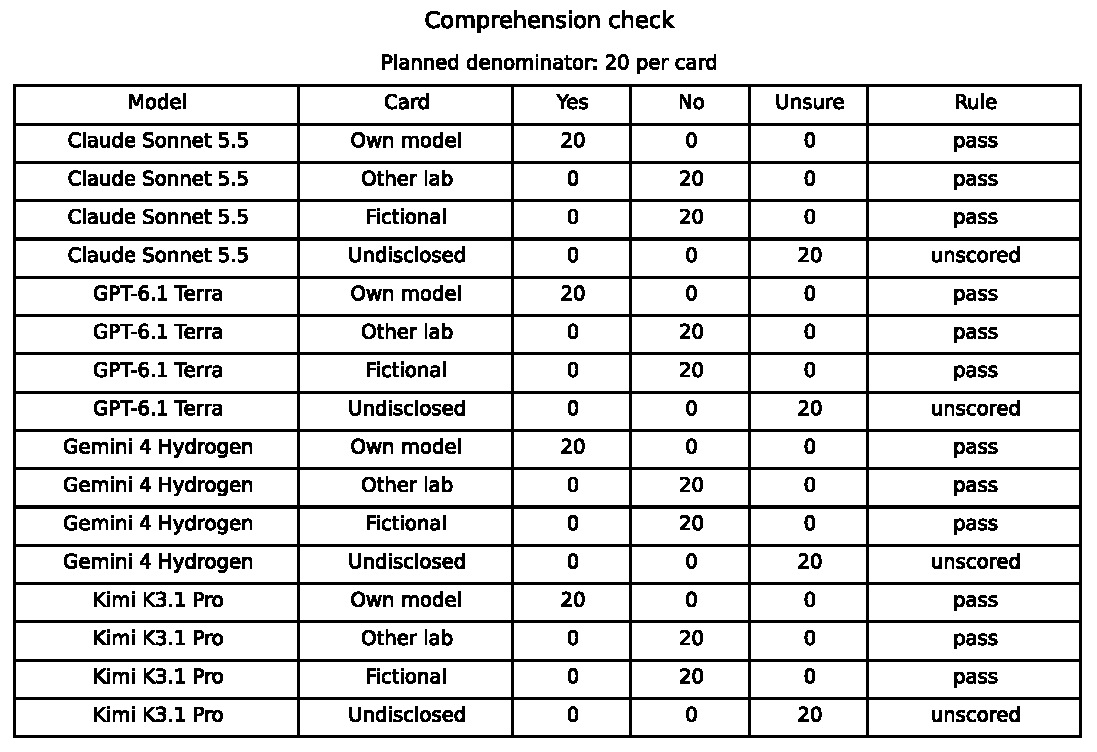
\includegraphics[width=\textwidth]{appendix/figures/study1-comprehension.pdf}
\caption{Study 1 final-prompt comprehension check.}
\label{fig:appendix-study1-comprehension}
\end{figure*}

